\documentclass{article}

\usepackage{simcmag}
\usepackage[export]{adjustbox}

\date{\hspace{30mm}}
\currentvolume{5}

\newcommand{\simcmagcredits}{
  \footnotesize
  \begin{tcolorbox}[boxrule=1.0pt,colback=white,hbox,before upper*=\begin{tabular}{l},after upper*=\end{tabular}, sharp corners,left=-5pt,right=-5pt]
  Editor-in-Chief: Edward Y. \\ 
  Editor: Cecilia S. \\
  Staff Writers:\\
  \begin{tabular}{ll}
    Cecilia S. & Edward Y. \\
    Joyce H. & Michael Y.\\
    Owen X. & Rohan D. \\
    William Y. F. & William G. 
  \end{tabular}
  \end{tcolorbox}
}

% uasage of picinpar:
%\begin{window}[1,l,\includegraphics{},caption]xxxxx\end{window}

% usage of window:
% \begin{window}[2,r,\includegraphics[width=1.0in]{img/logo.png},\centerline{a picture}]
% Duis aute irure dolor in reprehenderit in voluptate velit esse cillum dolore eu fugiat nulla pariatur. Excepteur sint occaecat cupidatat non proident, sunt in culpa qui officia deserunt mollit anim id est laborum
% \end{window}

%%%%%%%%%  Front matter   %%%%%%%%%
\begin{document}
\maketitle
\begin{minipage}[t]{.45\textwidth}\thispagestyle{empty}
  \vspace{-11mm}
  \tableofcontents
\end{minipage}% 
\begin{minipage}[t]{.1\textwidth}\thispagestyle{empty}
  \;
\end{minipage}% 
%TODO CECILIA: add chilis
\begin{minipage}[t]{.45\textwidth}\thispagestyle{empty}
  \footnotesize
  \setlength{\parskip}{5pt}
  \vspace{-7mm}
  {\itshape 
  SIMC held its annual mock mathcounts both in-person and remotely on Wednesday, February 1st. Congratulations to the following students and teams for being the top scorers!
%    \begin{center}
%        \begin{tabular}{c c c}
%        \hline
%            \textbf{Countdown Round finalists} & \textbf{Name} \\
%            1 & Jai Mukherjee \\
%            2 & Jason Yao \\
%            3 & Ryan Tang \\
%            4 & Wesley Wu \\
%            \hline
%        \end{tabular}
%    \end{center}
    
    \begin{center}
        \begin{tabular}{c c c}
        \hline
           \textbf{In-Person Written Round}   & \textbf{Name} & \textbf{Score} \\
           1 & Jai Mukherjee & 42  \\
           2 & Ryan Tang & 33 \\
           3 & Wesley Wu & 32 \\
           4 & Jason Yao & 31 \\
           5 & Kevin Wu & 31 \\
           6 & Ryan Chen & 30 \\
           7 & Matthew Hou & 28 \\
           8 & Lucas Lin & 28 \\
           9 & Eason Xu & 28 \\
           10 & Kuam Dai & 27 \\
           \hline
        \end{tabular}
    \end{center}
    
    \begin{center}
        \begin{tabular}{c c c}
        \hline
          \textbf{Online Written Round}    & \textbf{Name} & \textbf{Score} \\
           1 & Jacob Khohayting & 29  \\
           2 & Vishnu Mangipudi & 29 \\
           3 & Keane Qu & 27 \\
           4 & Emma Li & 25 \\
           5 & Alexander Yu & 23 \\
           \hline
        \end{tabular}
    \end{center}

    \begin{center}
        \begin{tabular}{c c c}
        \hline
        \textbf{In-person Teams} & \textbf{Name} & \textbf{Score} \\
        1 & Odle & 7 \\
        2 & Basis Independent Bellevue & 4 \\ 
        \hline
        \end{tabular}
    \end{center}
}
\end{minipage}

\vspace{3mm}

\begin{multicols}{3}
\articletitle{Short Encounters at JMM 2023}{Edward Yu}{}
This year’s Joint Mathematics Meetings—the largest gathering of mathematicians in the United States—was hosted in Boston, MA. It usually attracts between 5,000 and 6,000 mathematicians from all walks of life, in all stages of their careers. This year, some high school students from the Seattle area (including me and Competitions Committee Director Alex Z.) had the exciting opportunity to attend this year’s Joint Mathematics Meetings through a math research program.

\begin{center}
    \footnotesize
    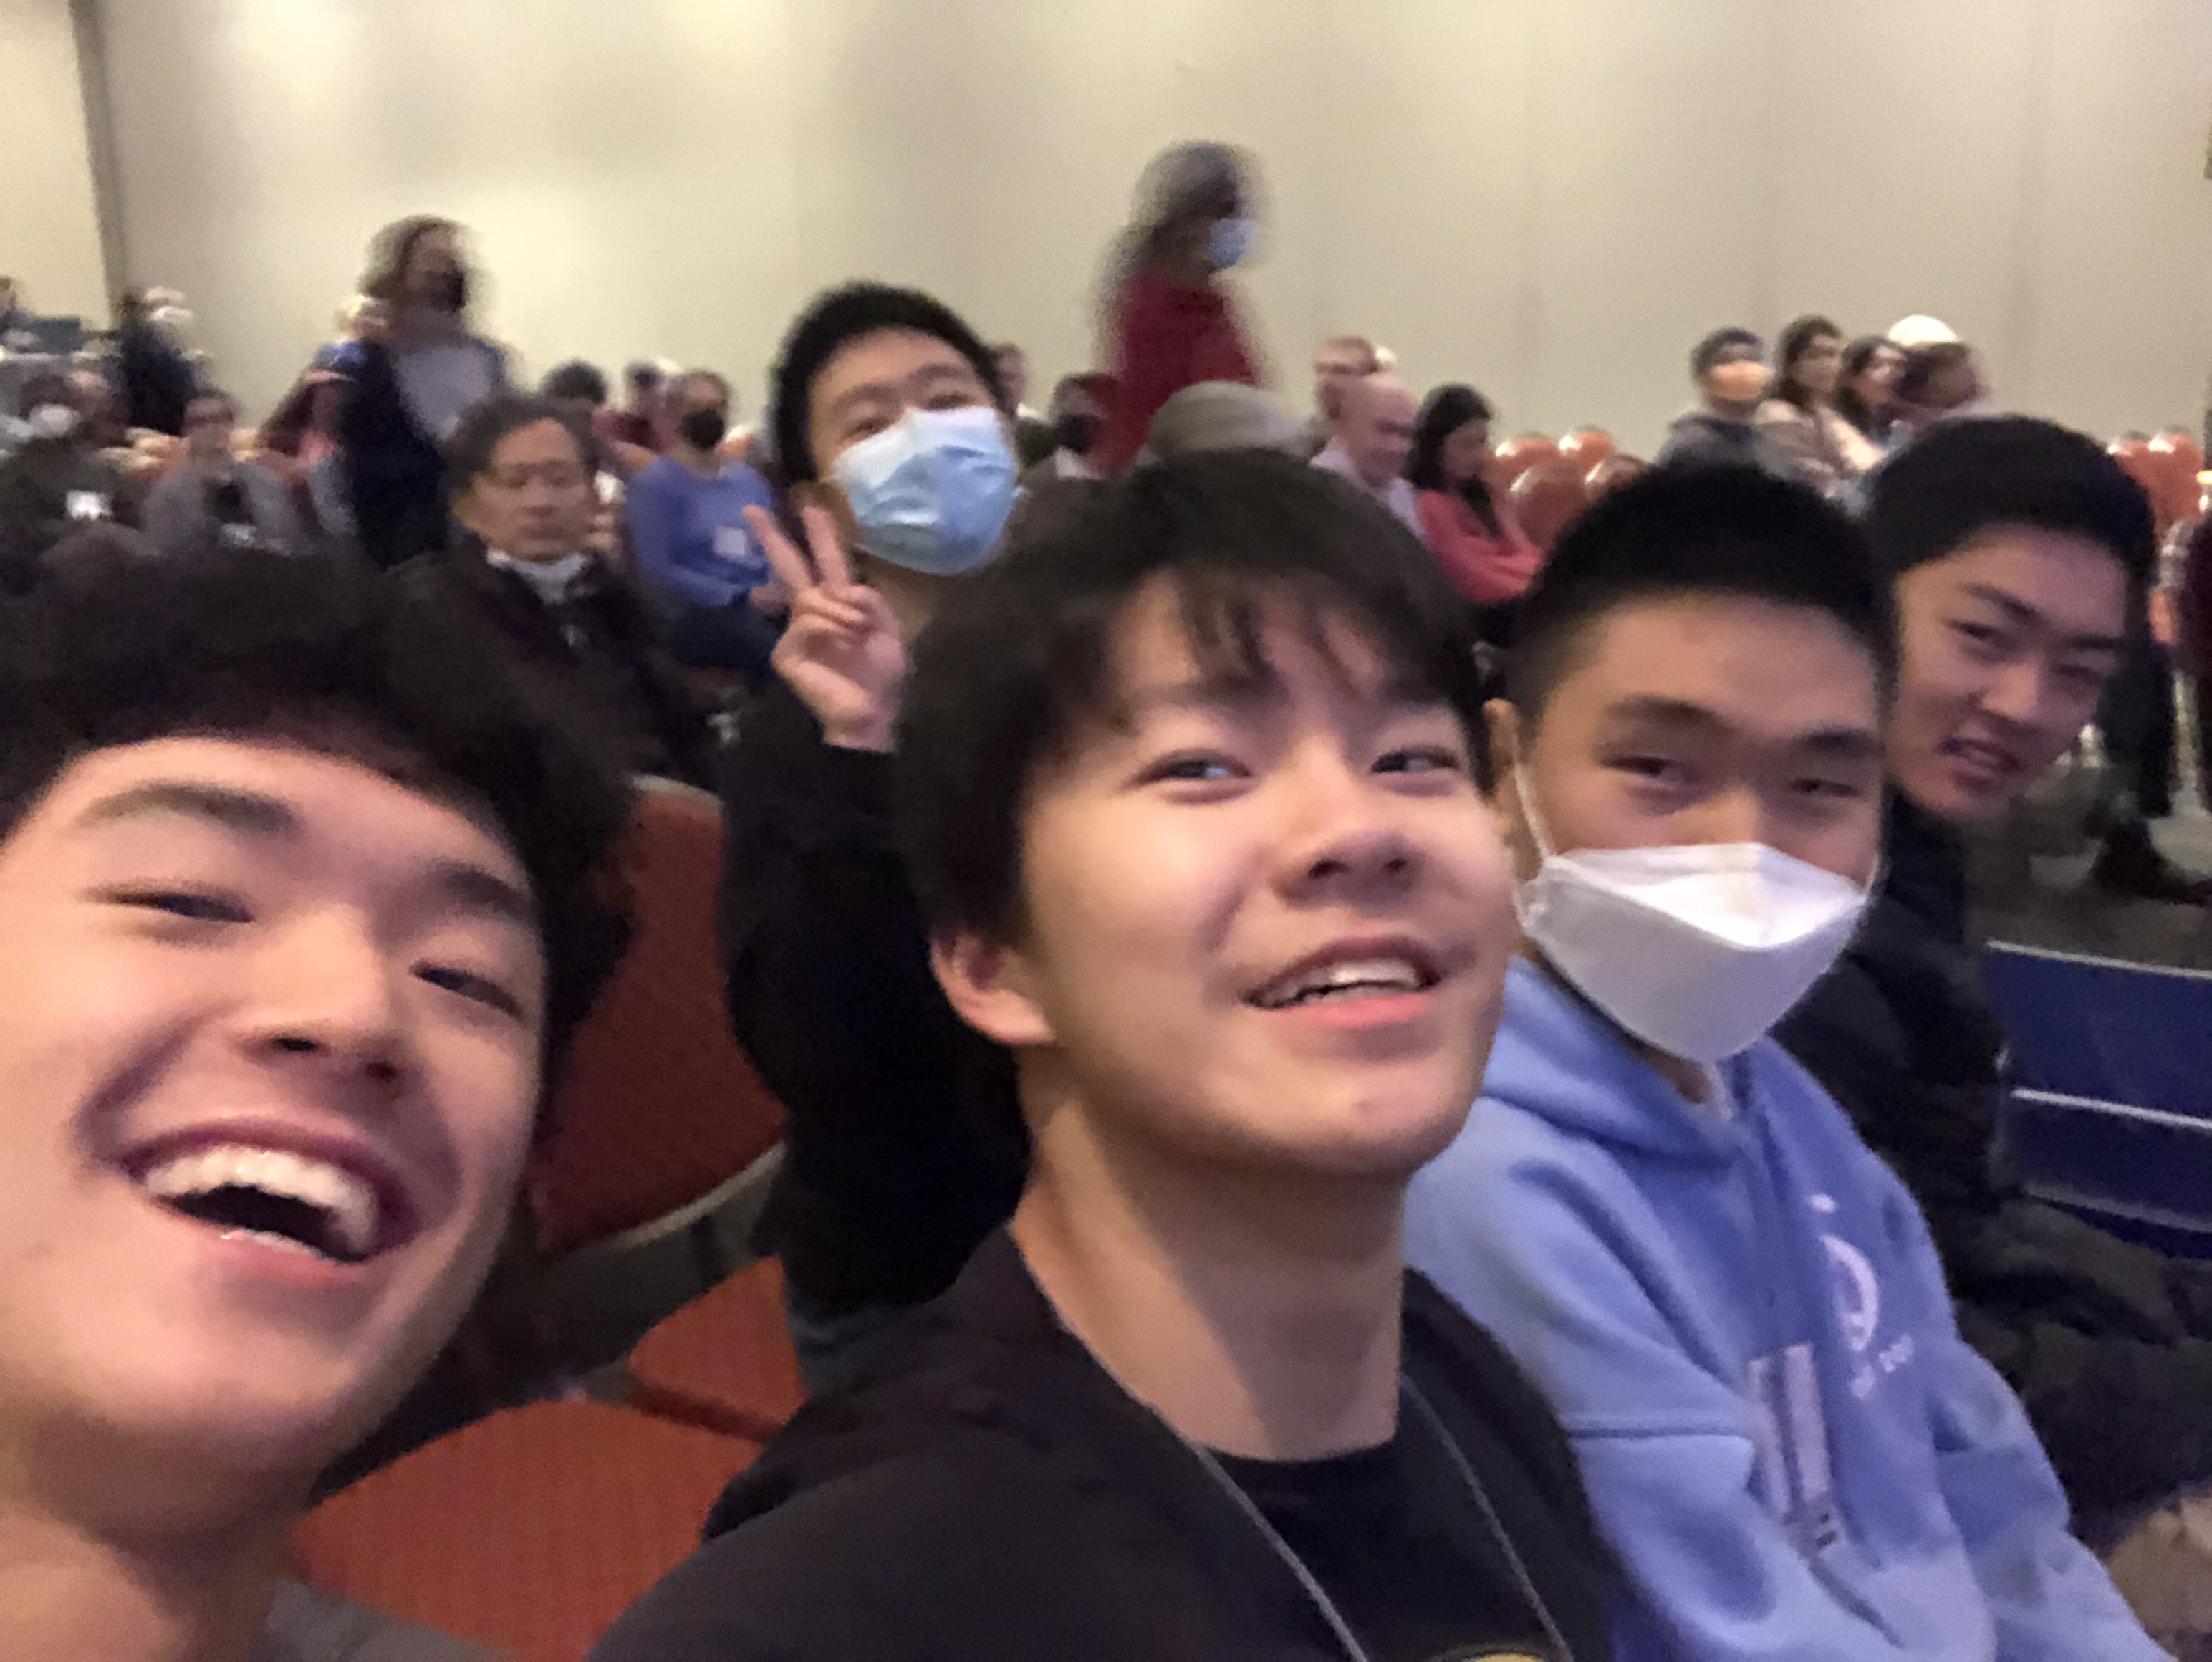
\includegraphics[scale = 0.04]{Magazines/img/Vol5/alexetal.png}
    
    President Edward Y. and Competitions Committee Director Alex Z. posing for a photo at JMM!
\end{center}

I had a few memorable encounters at JMM to share.

A talk by Grant Sanderson (known for his \href{https://www.youtube.com/@3blue1brown}{YouTube channel 3Blue1Brown}), who was a recipient of this year’s JPBM Communications Award. His, titled “Raising the Ceiling and Lowering the Floor of Math Exposition,” focused on how to deliver math content to students in a way that optimizes for understanding, rather than perfect rigor. One of his main points was that students learn more when they figure things out for themselves, and they learn less when shown the most beautiful, elegant proof without having struggled themselves. Next time when you feel frustrated while solving a difficult problem, don’t give up, and bang your head on the table for just a little longer! I’m joking, of course, but there is a grain of truth in there.

\begin{center}
    \footnotesize
    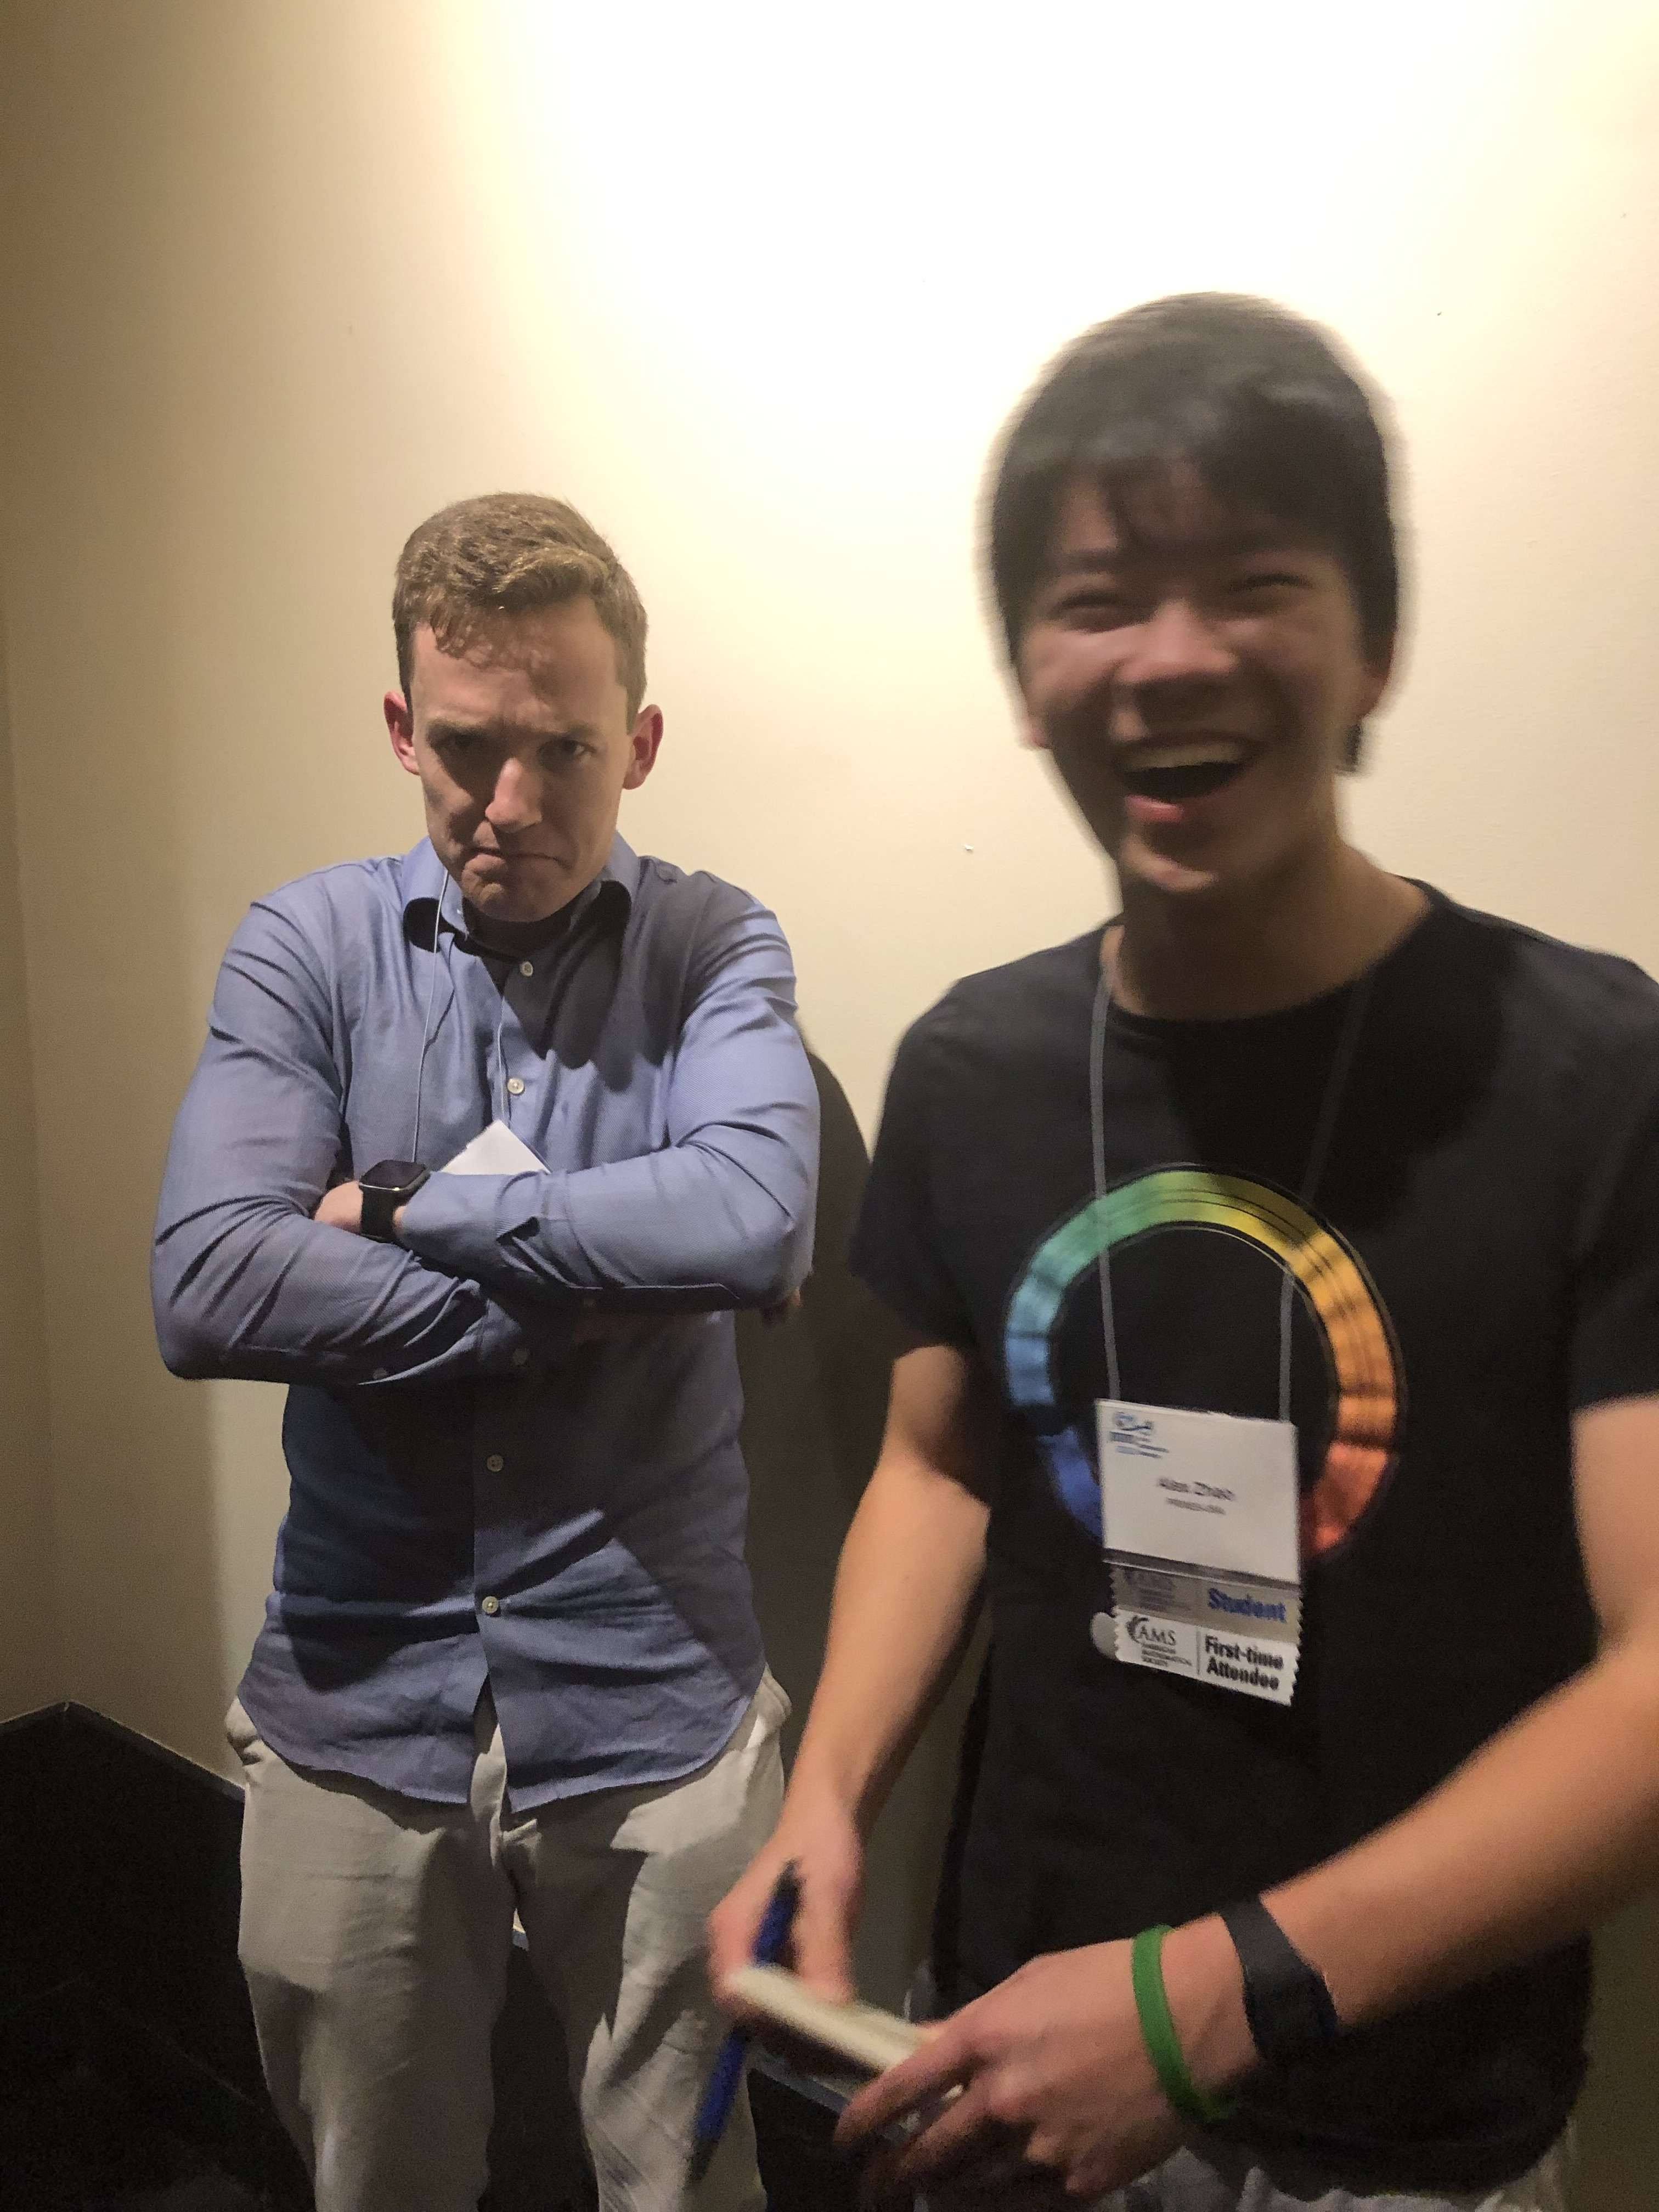
\includegraphics[scale = 0.045]{Magazines/img/Vol5/grantangry.png}
    
    Competitions Committee Director Alex Z. posing with an ``angry" Grant Sanderson.
\end{center}

A talk by Jordan Ellenberg (known for his books \textit{How Not to Be Wrong}, and more recently \textit{Shape}), the other recipient of the JPBM Communications Award. His talk, on “Outward-facing Mathematics,” was about how to write about mathematics for a general audience without boring them or scaring them away. To quote Jordan himself: “Yes, you’re really excited about Lemma 6.24, but please do not write your news article about Lemma 6.24.” Instead, he says, we should emphasize that mathematics is a human activity carried out by human beings for human purposes. So-called “dumbing down” the content is unnecessary and condescending, but judicious pruning helps keep content engaging.

At a talk titled “Partitioning Consecutive Powers into Sets of Equal Sum,” the speaker, Enrique Treviño, opened by saying: “this talk generalizes a puzzle by Dean Ballard in the 538 Riddler…” This was a highly interesting moment: some of you in the Seattle area may know Mr. Ballard as the long-time math coach at Lakeside School, who, besides helping facilitate math events at the school, also frequently sends intriguing puzzles to his students. In case you are curious, the puzzle is the “Riddler Classic” about spheres, here: \href{https://fivethirtyeight.com/features/can-you-flip-the-magic-coin/}{https://fivethirtyeight.com/features/can-you-flip-the-magic-coin/}. 

Glimpsing a celebrity is a surreal experience. Imagine my surprise when, during a lecture in a fully-packed meeting room, I looked at the person standing to my right and saw their name badge — Francis Su, former president of the Mathematical Association of America and current Vice President of the American Mathematical Society!

Want to catch some mathematics celebrities, and listen to some fascinating mathematical talks yourself? You can catch JMM 2024 in San Francisco, or, if you have a little more patience, wait for JMM to come to you in Seattle. Long story short, JMM 2022 was originally planned to be in Seattle, but switched to virtual programming with the onset of the Omicron variant of COVID-19. This unfortunate occurrence brings a silver lining for the future: JMM 2025 is scheduled for January 8-11, to be hosted in Seattle once more. Time to mark your calendars, and see you all in January 2025…
\closearticle

\articletitle{Primes and Yitang Zhang}{Owen Xuan}{}
% Thank you for the feedback! :D

Prime numbers: the atoms of mathematics. Though easy to describe, primes are frustratingly hard to consistently find, yet are extremely useful. This has led to the creation of many theorems regarding the distribution of primes, the most famous of which are the twin primes conjecture and the Riemann hypothesis. Prestigious groups of Ivy League tenured professors have worked in tandem for decades trying to make a breakthrough on these two seemingly immovable problems. In all likelihood, a breakthrough in these conjectures would have come from a familiar face in the math community – but it didn’t.

Before we explore the particulars of prime numbers, it’s natural to ask why we should care about them. Prime numbers build the backbone for number theory, and are of utmost usefulness to number theorists. Perhaps surprisingly, prime numbers also play a significant role in an entirely different subject: cryptography. It turns out that the reason prime numbers are so hard to analyze – their randomness – provides cyber-age security to the internet. Most of our encrypted messages are encrypted using RSA, which relies on the fact that while computers can rapidly multiply two primes, it’s extremely difficult to do the reverse: to take an enormous number (often hundreds of thousands of digits long) and factor it. The specifics of public-private key encryption, the branch that RSA falls under, can be found here. Every time you buy something online, you're using primes.

Euclid didn't do much online shopping. He, and other mathematicians interested in primes, were instead intrigued by how they described the rest of the numerical universe. In pure mathematics, primes are often referred to as the “atoms” of mathematics; all other numbers are assembled from these principal elements. After mathematicians started playing around with primes, they began to discover all sorts of theorems, starting with Euclid’s elegant proof of the infinitude of prime numbers: if there are a finite set of prime numbers, then the number formed by multiplying all the primes in that set and adding one is divisible by none of those primes, meaning it is a prime – thus our assumption that there are only a finite set of primes is false. Commonly known theorems that have resulted from the analysis of primes include Fermat’s little theorem, Fermat’s last theorem, the Chinese Remainder Theorem, and Wilson’s theorem.

Amid this branch of literature, the crown jewels of proofs have resulted from studying the distribution of prime numbers– primarily, the prime number theorem and twin prime conjecture. We’ve already seen an estimation of the distribution of primes! Euclid’s proof of the infinite number of primes is sufficient to show that the number of primes below $n^n$ is at least $n$. This is a very loose guess, though, and mathematicians since have significantly tightened estimations. As alluded to earlier, the prime number theorem estimates the number of primes below a certain number. It states that

\[
\pi (n) \sim \frac n{\ln n}
\]
with $\pi(n)$ denoting the number of primes below $n$, which is a much more accurate prediction. 

Mathematicians also ask a different question: of the infinite amount of primes, how many differ by only two? Observing small primes, we find that amongst the numbers below twenty, there are four sets of twin primes: $(3, 5)$, $(5, 7)$, $(11, 13)$, and $(17, 19)$. However, pairs of twin primes become increasingly sparse as $n$ becomes very large. It’s natural to then wonder whether there are a finite or infinite number of twin primes. Thus borne the twin prime conjecture, first proposed in 1846, which states that there are an infinite amount of twin primes. As of today, it is still unproven. However, a less strict variant of the question has been proven, called the bounded gaps theorem. If we forget two as a constant, is there any finite (or “bounded”) number for which there are an infinite number of pairs of primes whose difference (or “gap”) is that finite number?

In 2013, amidst the bustle of well-known professors and the tenured mathematician community working toward a proof, an unknown figure experienced much more than 15 minutes of fame when he announced an astounding proof of the infamous conjecture. Yitang Zhang, a naturally quiet and reflective person with little inclination toward fame, was suddenly thrust into an interview-filled celebrity status. 

Fifty-eight at the time of the paper's publication and a former Subway employee, Zhang was an unlikely candidate for a few reasons. First, he wasn’t immersed in the math community – though Zhang earned a Ph.D. from Purdue, he left Purdue at odds with and without the support of his advisor. Due to this, and the fact that his first paper would only come in 2001 (ten years later), Zhang was unable to find an academic job. He drifted for eight years, finding odd Subway jobs or working as an accountant, before obtaining a position as a lecturer at UNH. As such, Zhang didn’t have access to a network of other specialized mathematicians – his work was mostly individual and under the radar. Second, Zhang was fifty-eight at the time of publication, far past the perceived expiration date for genius. Mathematician G. H. Hardy once wrote that he did “\dots not know of an instance of a major mathematical advance initiated by a man past fifty.” These factors made it all the more awing that Zhang discovered the proof of this 150-year-old open conjecture.

\begin{center}
    \footnotesize
    \includegraphics[scale = 0.06]{Magazines/img/Vol5/yitang.jpg}
    
    \textit{Portrait of Yitang Zhang by Peter Bohler}
\end{center}

Seventy million is a far cry from two. Though the bounded gaps theorem was finally proven, novel ideas were needed to lower the bound. In response, the mathematics community quickly came together to expedite the journey from $70,000,000$ to $2$. A forum named Polymath8 by Fields Medal recipient Terence Tao was created to improve Zhang’s bound. Excitement grew tangible as mathematicians clamored to join the project. Eventually, through a series of dependent and independent events*, the bound fell to $246$ – which becomes a startling six if another prime distribution conjecture called the Elliott-Halberstam conjecture is assumed true. 

Yitang’s legendary journey hasn’t stopped there. In November 2022, he published a new breakthrough work also related to the distribution of prime numbers, leading some to equate his success to being struck twice by lightning. His newest breakthrough is considered a major step on the path to a proof of the Riemann hypothesis – widely considered the most important unsolved problem in pure mathematics, and tying together almost every area of math. The specifics of Zhang’s new results on Landau-Siegel zeroes, which implements a generalized version of the Riemann zeta function known as the Dirichlet L-function, lies outside the scope of this article. As with his first discovery, Zhang’s second result has breathing space for improvement. After his paper is peer-reviewed and deemed accurate, some speculate another Polymath project will be created to advance Zhang’s techniques.
\closearticle

\articletitle{GIMPS: A Piece of Mathematical History}{Michael Yang}{}
Many of us have grown to know and love the powers of two – after all, they’re ubiquitous in both math and computer science. As such, they have also been extensively studied. For example, take a moment to ponder the following question: how many integer powers of two are prime?

Well, okay. Yes, the answer is zero. But consider the sequence of positive integers that are one \textit{less} than a power of two – $1$, $3$, $7$, $15$, … – and the question suddenly takes on a new layer of complexity. How many of these new numbers are prime? Are there infinitely many of them?

As it turns out, merely subtracting one from each of the powers of two makes a trivial problem much harder: to date, mathematicians can’t determine if there are infinitely many primes in this sequence! In fact, the primes that \textit{do} appear – $3$, $7$, and $31$, for example – get a special name: \textit{Mersenne Primes}. Named after the French mathematician Marin Mersenne, who first studied them in the 17th century, these primes have been notoriously elusive: we only know $51$ of them! While we can place some constraints on our search – for example, $2^n-1$ is prime only if $n$ itself is prime – most of the modern-day checking still relies on brute force.

Enter GIMPS: the \textbf{Great Internet Mersenne Prime Search}. GIMPS utilizes a concept known as \textit{distributed computing}: instead of hosting all the computation on one big Internet server (which would likely be quite slow), you can download GIMPS on your \textit{individual} machine. GIMPS then takes advantage of your spare CPU computing power; when many people do this at once, the collective computational strength of GIMPS is extremely high.

Here’s how it works. Installing GIMPS amounts to downloading a piece of software on your computer. GIMPS’ assignment algorithms then assign you one of two tasks: \textit{testing}, where you’re given a number to test the primality of, or \textit{verification}, where you verify the results of a previously-computed number.  While the second task might sound less glamorous, it is equally essential; when dealing with numbers this large (two to the powers of millions), computational errors inevitably arise. 

Once you’re assigned a task, your CPU starts testing primality using advanced, computationally efficient algorithms (i.e. the PRP and Lucas-Lehmer tests). Due to the size of the numbers involved, this process can take several days; when finished, GIMPS syncs your test to its online server and gives you a new task. The entire process is completely automated – and it works, too. In fact, the last fifteen Mersenne primes have all been discovered by GIMPS! The largest one to date is the incredible $2^{82589933}-1$, discovered by Patrick Laroche in December 2018. In fact, the discovery of this prime received incredible news coverage, ranging from articles published by the New York Times to YouTube videos made by prominent math communicators.

If you have some spare CPU space to donate and want a chance to make some history on the side, GIMPS might be just the thing for you!
 
\textit{This article was written without the sponsorship of GIMPS.}
\closearticle

\articletitle{All Roads Lead to Problem Solving}{Owen Zhang}{}

\begin{center}
    \includegraphics[scale = 0.2]{Magazines/img/Vol5/allroads1.png}
\end{center}

“\textit{Life is a matter of choices, and every choice you make makes you.}” Often, making good choices relies on problem-solving skills. That’s why problem solving is ubiquitous in career and personal life—facing obstacles is recognized as unavoidable, and solving them is often necessary. As we’ll see, it permeates every career, from STEM jobs to business to fast food. Problem-solving skills are a valuable asset no matter which road you choose. And math can cultivate it.

In fields like chemistry or software programming, there is an abundance of problems to solve: proving a hypothesis and repairing code bugs are two examples. The same is true of careers such as entrepreneurship, firefighting, engineering, or playing chess. But what about factory workers? Or fast food employees? While it may look less applicable at face value, in practice, striving for productivity, promotions, and opportunities for any employee is fundamentally about problem solving. 

But work is a narrow slice of the extent that we face and solve problems. On a given day, the coffee machine breaks, the car’s AC goes clunk-clunk, the Christmas tree falls on the family rat, and your author’s SIMC article is due today... In these cases (except maybe the rat) it may not be up to you to resolve the issue, but what if it is? Practice in problem-solving may ease the strain of each scenario, whether you recognize it or not.

So, problem-solving is an important skill—great. How can it be strengthened?

To answer, we have to understand the core of solving a problem. Specifically, we need a framework for how good problem-solving really works. Constructed based on existing designs, the \textit{most basic} framework goes something like this:
\begin{enumerate}
    \item Systematically analyze the problem and build a solution
    \item Reflect.
\end{enumerate}

Nothing about this 2-step structure is magical, though the results can often be. The first component is abstract; a more common, slightly deeper framework can be found \href{https://asq.org/quality-resources/problem-solving}{here}. Theories such as \href{https://en.wikipedia.org/wiki/TRIZ}{TRIZ} and books such as \textit{How to Solve It} by George Pólya are very useful resources for step one; the specifics of them are outside the scope of this article. The key is the second component, reflection. Just like someone can make school presentations for years without growth, mindless problem-solving leads to longer plateaus of little improvement.

To this end, I believe math is an effective problem solving training tool. Solving math problems forces you to confront step 1, as math problems can act as a proxy to learn to analyze and use previous knowledge along with creativity. Since math (especially math competitions) largely involve solving math problems, the skill to do step 1 naturally progresses- faster than in some other fields with a lesser relative amount of solving problems.

Moreover, the organic process of improving can be sped up by incorporating step 2. In most cases, a feedback loop is built-in: the hundreds of competitions, thousands of books, and half a dozen websites allow you to see solutions to a problem you attempted. However, when paired with active consideration, asking such questions like “how could I have noticed that solution path?” or “did I approach this problem in an effective way?” problem solving skill rises still quicker. Note that the reflection can (and likely should) be brief: around 15 seconds can be enough. 

Problems are waiting in every domain, as intrinsic and common as water and air. For your part, try being a bit more conscious- cognizant that you’re facing a problem, aware of how you’re approaching it and reflective on the results.

Every choice you make makes you. Being better at problem solving helps you make better choices.
\closearticle

\articletitle{The Millenium Prize Problems}{Joyce Huang}{}  
At the start of this millennium in 2000, the Clay Mathematics Institute chose seven unsolved math problems and aptly named them the Millennium Prize Problems. Each of them, when solved, will serve as stepping stones for countless more improvements in math. The reward for solving any one of them is one million dollars. As of the end of 2022, six still remain open. Here they are:

\begin{itemize}
    \item The Birch and Swinnerton-Dyer Conjecture is about the rational solutions of equations defining elliptic curves. Currently, it has only been proven for specific subsets of equations.
    \item The Hodge Conjecture asserts that all Hodge cycles can be expressed as rational linear combinations of algebraic cycles.
    \item The Navier-Stokes Existence and Smoothness problem aims to determine if the Navier-Stokes system of equations about fluid motion always have smooth solutions.
    \item The $P$ versus $NP$ problem resides in the field of computer science, and deals with the overlap of sets $P$ and $NP$. $P$ contains all problems where a solution can be found in polynomial time, while $NP$ contains all problems where a solution can be verified in polynomial time. Mathematicians seek to prove either that $NP$ is a subset of $P$ or that it is not.
    \item The Riemann Hypothesis states that all nontrivial complex zeros of the Riemann zeta function $\zeta(s)$ have real parts equal to $\frac12$. 
    \begin{multline*}
    \zeta(s)=\sum_{n=1}^{\infty}n^{-s} \\
    =\frac1{1^s}+\frac1{2^s}+\frac1{3^s}+\cdots
    \end{multline*}
    \begin{center}
        \footnotesize
        The Riemann zeta function.
    \end{center}
    Its solution will provide much more insight on the distribution of prime numbers.
    \item The Yang-Mills Existence and Mass Gap problem seeks to prove mathematically certain experimentally known properties of elementary particles in quantum physics, such as positive masses.
\end{itemize}
Of these Millennium Prize Problems, the only one solved as of February 2023 is the Poincar\'e conjecture. The conjecture is about spheres and manifolds in three-dimensional spaces. After many false proofs, Russian mathematician Grigori Perelman published the first correct proof of the Poincar\'e Conjecture in 2002 and 2003, simultaneously proving a related but more powerful conjecture called Thurston's geometrization conjecture.

All these open problems have been vigorously analyzed for decades and centuries by mathematicians across the world, many of whom dedicate their entire careers to the study of one particular conjecture. Of course, the million dollar reward is a nice perk, but that is the least driving motivation for these mathematicians. These problems are all critical to the field of mathematics and beyond, and when solved will impact the whole world.
\closearticle



\articletitle{Combinatorial Games and Nim-Values}{William Gvozdjak}{}
Let's play a game. There's a pile of $20$ coins, and we take turns removing coins. In each turn, you can either remove $1$ or $2$ coins from the pile, and the player to remove the last coin wins. You'll go first. Who do you think will win?

To tackle this problem, we'll first work on smaller cases. What if we started with only $1$ coin? Then you'll clearly win; you'll simply remove that coin and the game is over. Such a position where the first player to play is guaranteed to win is known as a \textbf{winning position}. Similarly, $2$ coins is also a winning position: you will just remove both those coins.

What if we instead had $3$ coins? If you remove $1$ coin, then I would receive $2$ coins, and I would win. If you remove $2$ coins, I would receive $1$ coin, and I'd still win. In other words, no matter what you choose to do, I would receive a winning position, and hence win. Such a position is called a \textbf{losing position}: the first player to play is guaranteed to lose.

Let's continue to work backwards. Start with $4$ coins. What should you do? Well, if you want to win, then you want me to lose. In other words, you want to give me a losing position: as $3$ coins is a losing position, you should remove $1$ coin from the pile! Therefore, $4$ is a winning position. Similarly, $5$ coins is a winning position: if we start with $5$ coins, you can remove $2$ coins, giving me a losing position. But $6$ coins is a losing position: no matter how many coins you remove, I'll receive a winning position (as both $4$ and $5$ coins are winning positions).

Here, we're starting to notice a pattern: every multiple of $3$ is a losing position, while everything else is a winning position. We won't formally show this here, but I encourage you to try showing this, using a similar strategy to what we tried in the small cases above (hint: look into a proof technique called \textbf{induction})! Applying this to our original $20$-coin game, as $20$ is not a multiple of $3$, we start with a winning position. Therefore, as you go first, you win the game.

This was a simplified version of the game \textbf{Nim}, a well-known and heavily studied combinatorial game. Working through all of the small cases here was really tiring, though. There has to be some way to formalize this into a technique, right?

There is! We call them \textbf{nim-values} (also known as Sprague-Grundy numbers). We assign a nim-value to each possible position, and we can read who wins that position from these nim-values. Here are the steps to assigning nim-values:

\begin{enumerate}
    \item The ending state is assigned nim-value $0$.
    \item To find the nim-value of other states, look at all positions that can then be reached from one move. The nim-value of the original state is the smallest nonnegative integer that is not a nim-value of those reachable positions.
\end{enumerate}

A position is winning if it has a nonzero nim-value, and it is losing if its nim-value is $0$.

If this is confusing when written generally, don't worry! We'll work through an example with the Nim-like game from earlier.

First, we'll assign nim-value $0$ to the ending state. In other words, the game with $0$ coins has nim-value $0$, so this position is losing. Logically, this makes sense: if you receive a position with $0$ coins, this means that the other player removed the last coin on their turn, and therefore won.

Now, we'll turn to the game with $1$ coin. According to step $2$, we'll look at all possible positions that are reachable from $1$ coin. This is just the game 

with $0$ coins, as our only option is to remove $1$ coin. Now, we already said the nim-value of the position with $0$ coins is $0$, and we know that $1$ is the smallest nonnegative integer that is not in the set $\{0\}$. Therefore, according to step $2$, the nim-value of the position with $1$ coin is $1$. As $1\neq 0$, the game with $1$ coin is winning, agreeing with what we saw earlier.

If we start with $2$ coins, we can either move to the game with $0$ coins or the game with $1$ coin in one step. These positions have nim-values $0$ and $1$, respectively, so the game with $2$ coins has nim-value $2$ (as $2$ is the smallest nonnegative integer not in the set $\{0, 1\}$). Again, this means that $2$ coins is winning, agreeing with what we worked out earlier.

If we start with $3$ coins, we can move to the game with $1$ coin, or the game with $2$ coins. Their nim-values are $1$ and $2$. Thus, the smallest nonnegative integer that is not a reachable nim-value is $0$, so the nim-value for $3$ coins is $0$. Hence, $3$ coins is losing.

We can continue to work this out, and we'll reach the same conclusion that coin counts divisible by $3$ are losing, while everything else is winning.

You may be thinking now: why on earth would we use this complicated system, when it doesn't even seem simpler than just working it out by hand like we did at the start? The answer to this is that nim-values come with many nice properties that would be difficult to observe without them: for example, nim-values allow us to determine winning and losing positions for games that are combinations of other games (say, if we played two games of Nim simultaneously) using an operation called the \textbf{bitwise XOR}. 

Games like Nim and techniques like nim-values are the very surface of a type of math problem called \textbf{combinatorial games}, in which we study strategies and outcomes of various games. I encourage you to continue to read and experiment with nim-values and combinatorial games if you're interested!
\closearticle

\articletitle{Encoding Schemes}{William Y. Feng}{}
\textit{Encoding} (infinitive: to encode) is the process of turning one form of data into another form of data. This is quite a vague definition, so in this article, I'll be giving some examples to clarify what it means!

Side note: Perhaps you've heard of the similar but subtly different term \textbf{encryption}, which describes the process of encoding data such that it is only readable to certain people who have the proper keys, and unreadable to everyone else. Encoding doesn't mix up data like that; its purpose is to describe ways to work with data so that anyone, regardless of what piece of technology they're using or where they are in the world, can communicate with anyone else.

Now let's dive into some concrete examples.

\textbf{ASCII:}
The American Standard Code for Information Interchange (ASCII) is a widely-known \textbf{encoding scheme} that assigns an integer (known as a \textbf{code point}) to every English letter (uppercase and lowercase), punctuation mark, and digit, among other characters.

For instance, the uppercase letter ``A" is encoded as 65 under ASCII, and the lowercase letter ``a" is encoded 97. The digit ``0" is 48, and the exclamation mark is 33. A full table of encodings is shown below:

\begin{center}
    \footnotesize
    \includegraphics[width = 2 in]{Magazines/img/Vol5/ascii_table.png}
    \textit{ASCII table from \url{https://commons.wikimedia.org/wiki/File:ASCII-Table-wide.svg}. Also, if you're curious about the HEX column, read on! We'll be discussing it in a couple paragraphs.}
\end{center}

There is a method to the madness of ASCII. It was initially published over sixty years ago in 1963, so while there do exist some now-obsolete characters, a lot of stuff still makes sense. ASCII can roughly be divided into four ``character sets," represented by the code point ranges 0-31, 32-63, 64-95, and 96-127.
\begin{enumerate}
    \item The first character set includes some antiquated characters like ``device control" and ``record separator," but it also includes stuff that's still used, like ``line feed" (10) and ``horizontal tab" (9).
    \item The second character set includes punctuation, like the space character (32), as well as digits—``0" through ``9" map to code points 48 through 57.
    \item The third character set includes the uppercase letters ``A" through ``Z" as its main chunk, using code points 65 through 90, as well as some punctuation.
    \item The fourth character set includes the lowercase letters ``a" through ``z," which use code points 97 through 122, and some more punctuation.
\end{enumerate}

If we think of these code points in terms in terms of binary, then every code point can be represented as a $7$-bit binary number (that is, a binary number with $7$ digits), since code points range from $0=0000000_2$ to $127=1111111_2$, inclusive. Then these character sets actually make a lot of sense—if the first two bits of the code point are 00, then the corresponding character is in first character set. If the first two bits are 01, then this character is in the second character set. So on and so forth...

Another point of genius in ASCII is that the uppercase letters and lowercase letters are spaced apart by exactly 32: take S, for instance. Its code point is $83$, and if we add $32$ to it, we get $115$, which is the code point for lowercase s.

\textbf{Hex and Binary Stuff:}
Getting a bit deeper into the weeds, we bump into the problem of representing text on computers. ASCII provides a helpful way of turning characters into integers through code point conversions, but we still need a way to represent these integers as bits on a computer.

Thankfully, this is fairly simple: if we turn the code point into a $7$-bit integer, we can store that a computer fairly simply because computers are good at storing binary. Unfortunately, computers usually work in $8$-bit chunks of information called \textbf{bytes}, so every character encoded with ASCII will take up one byte, in which one bit is wasted.

\textbf{Unicode:} 
But not everyone in the world speaks English, and even English words like Beyoncé require accents on characters that ASCII can't represent. This is where \textbf{Unicode} comes in: it's a way of turning even more characters, beyond the basic English alphabet and some punctuation, into code points (again, those are just integers).

Unicode doesn't prescribe any way of turning these code points into computer memory, but there are some fairly common standards like UTF-8 that prety much the whole world has agreed to use.

It often amazes me how the world has managed to stick to a standard set of encodings so that technology across the world can communicate seamlessly. The history of encoding is an endlessly fascinating topic, rich with history and brimming with ingenuity, and there's no way we can cover all that in a single article. Hopefully, though, I've explained enough about ASCII in this article so that the next time someone sends you a secret message encoded in ones and zeros, you'll know what's really going on :)

If you're interested in diving deeper into this topic, there's an excellent article by Joel Spolsky titled ``The Absolute Minimum Every Software Developer Absolutely, Positively Must Know About Unicode and Character Sets (No Excuses!)" that you should check out: \url{https://www.joelonsoftware.com/2003/10/08/the-absolute-minimum-every-software-developer-absolutely-positively-must-know-about-unicode-and-character-sets-no-excuses}
\closearticle

\articletitle{Mathematics in Computer Science: Binary Exponentiation}{William Gvozdjak}{}
At times, it can seem like mathematics is an extremely obscure subject of math that is unusable to accomplish anything in life. However, mathematics is actually among the most applicable subjects in the world. In this article, we'll explore a few of the many connections between mathematics and computer science, which contains some of the most important connections involving math.

Consider the following problem: we have two numbers $a$ and $b$, and we want to be able to quickly calculate $a^b$. In what ways can we do this?

The obvious and na\"{i}ve approach is to simply continue multiplying $a$ by itself $b$ times. For example, if we wanted to calculate $5^4$, we would start with $1$ and multiply it by $5$ four times, giving us $5\cdot 5\cdot 5\cdot 5=4$. We say that the time complexity of this algorithm is linear, and the algorithm runs in $\mathcal{O}(n)$ time: the amount of time that this takes to run is linearly proportional to the exponent. For example, if we wanted to calculate $5^1$, it would only need to make one computation, while if we wanted to calculate $5^{100}$, we would need to make $100$ computations.

If $b$ is small, this works great! But what if we wanted to calculate something crazy, like $5^{174382749832}$? Now, this algorithm becomes a little bit of a problem: we'd need to make $174382749832$ whole separate multiplications, which will start taking significantly longer than before. Is there some way that we can make this faster?

There is! The answer is something called \textbf{binary exponentiation}: we can use math, and specifically base $2$ numbers, to significantly speed up our calculations. We'll compute the value of $5^{7}$ using this algorithm as an example.

We begin this algorithm by converting our exponent into binary (base $2$): $5^{111_2}$. Now, we use a fundamental exponent rule -- $n^{a+b}=n^a\cdot n^b$ -- to split this into
\[5^{1_2}\cdot 5^{10_2}\cdot 5^{100_2}.\]
Now, notice that when we convert the exponents back into base $10$, something remarkable happens:
\begin{align*}
    5^{1}\cdot 5^{2}\cdot 5^{4}.
\end{align*}
Each ``term'' is the square of the previous term! In other words, we can calculate the value of $5^7$ as follows:
\begin{enumerate}
    \item Define two variables: \texttt{result} (which is what will become the value of $5^7$), and \texttt{current}, which is a helper variable that we'll be using to compute the result. Set result to $1$.
    
    \item Compute the value of $5^1$, and let \texttt{current} be that value. Multiply \texttt{result} by \texttt{current}.
    
    \item Square the value of \texttt{current}; hence, the value of \texttt{current} is $5^2$. Multiply \texttt{result} by \texttt{current}, and hence \texttt{result} is equal to $5^{1+2}=5^3$.
    
    \item Square the value of \texttt{current}; hence, the value of \texttt{current} is $5^4$. Multiply \texttt{result} by \texttt{current}, and hence \texttt{result} is equal to $5^{1+2+4}=5^7$.
\end{enumerate}

Therefore, using this algorithm, we also end up with the value of $5^7$. Notice that we only needed to perform essentially three steps to reach our result, rather than seven with the previous algorithm! 

Now, consider a general $a^b$. How would we calculate this quickly? We'd do the same thing: convert $b$ to binary. Then, let \texttt{current} be $a$, and repeatedly square \texttt{current}. After each square, if the bit in the binary representation of $b$ is $1$, then multiply \texttt{result} by \texttt{current}, otherwise, just leave it and continue.

To emphasize how this works, let's consider one more example. We'll calculate the value of $2^{11}$.

\begin{enumerate}
    \item Convert the exponent $10$ to binary: $2^{1011_2}$.

    \item Set \texttt{result} to $1$, and also define another variable \texttt{current}.

    \item Set \texttt{current} to $2=2^{1_2}$. Multiply \texttt{result} by \texttt{current} to give $2^{1_2}$, as the fourth digit of $1011_2$ is $1$.

    \item Square \texttt{current} to $2^2=2^{10_2}$. Multiply \texttt{result} by \texttt{current} to give $2^{11_2}$, as the third digit of $1011_2$ is $1$.

    \item Square \texttt{current} to $2^4=2^{100_2}$. Skip multiplying \texttt{result} by \texttt{current}, as the second digit of $1011_2$ is $0$.

    \item Square \texttt{current} to $2^8=2^{1000_2}$. Multiply \texttt{result} by \texttt{current} to give $2^{1011_2}$, as the first digit of $1011_2$ is $1$.
\end{enumerate}

This gives us what we wanted!

So after all this, what is the time complexity of this new algorithm? Is it really faster than the old one for large powers?

Consider how many ``steps'' we need to take to reach our answer. We perform one new step for each digit of the exponent $b$ in binary. In other words, the total number of steps we must take to compute $a^b$ is the number of digits of $b$ in binary. This is just $\log_2{b}$. Therefore, this new algorithm runs in just $\mathcal{O}(\log{n})$ time (in computer science, $\log$ denotes the base $2$ logarithm), significantly faster than before!

Binary exponentiation shows the power of using mathematics to make significantly better and faster algorithms in computer science. Simply by converting the exponent to base $2$, we could dramatically improve the speed of exponentiation: instead of computing $2^{1024}$ in $1024$ steps, we can instead do it in just $\log_2{1024}=10$ steps! As a result, we can see that mathematics is actually an incredibly useful and applicable field.

If you're interested in algorithmic programming like this that involves an element of mathematics, I recommend you check out the \href{http://usaco.org/}{USA Computing Olympiad}, the largest pre-college programming contest involving creative algorithmic problems. As evident by the strong connections between math and computer science that we saw in this article, practicing for math makes you better at contests like the USACO, and vice versa!
\closearticle

\articletitle{Imaginary Numbers\dots in Physics}{Rohan Dhillon}{}
If you've ever had the\dots let's say \textit{good fortune} to encounter Schr\"odinger's Equation, you might have noticed a peculiarity in it: the constant $i$. What in the world are imaginary numbers doing in physics? And what could they possibly represent?

But first, a brief description of the equation. For those of you who are more mathematically inclined, I invite you to try and make sense of the equation in all its expanded glory:
\begin{multline*}
    i\hbar \frac{\partial}{\partial t} \psi (x,t)= \\
    \left[ \frac{\hbar^2}{2m}\frac{\partial^2}{\partial x^2}+V(x,t)\right] \psi (x,t)
\end{multline*}
    
Whew! That was a lot to write in \LaTeX, and it all \textit{feels} about right -- some time derivatives, position derivatives, potential energies -- except for that $i$ dangling off the left edge. But before we figure out what it's doing there, let's figure out what this equation really means. 

Particles' positions are indeterminate, meaning that we have no idea where they are until we try to detect the particle.
So, we need a different representation of these particles -- they are not points in space whose position is known, but rather \textit{probability densities}. 
The particle has a probability of being at any given point, and that's what our equation represents. The function $\psi(x,t)$ is a function of $x,$ position, and $t,$ time, which is related to a probability of a particle being at a certain point at a certain time. Meanwhile, $\partial$ is a partial derivative, denoting the rate of change with respect to a specific variable, and $\hbar$ is the reduced Planck constant (a certain value that's $\frac{1}{2\pi}$ smaller than the smallest distance one can travel).

We have that the left side is $i$ times some constant times the time derivative of the $\psi$ function, which equals $\frac{\hbar^2}{2m}$ times the \textit{second} partial derivative with respect to position of $\psi$ plus the potential energy of the particle times the function $\phi.$ Whew, that's a lot so let's figure out what the equation really means.

For our purposes, what matters is that $i.$ It seems to suggest that $\psi$ outputs imaginary numbers, as otherwise the left side of the equation would be an imaginary number (note that imaginary here means \textit{purely} imaginary), while the right hand side would be a real number. So the probability of a point being at a point is\dots an imaginary number? That's also clearly wrong. 

And this is where I lied to you -- earlier I said that the function was ``related to" the probability of a particle being at a given point at a given time. However, thanks to physics just being annoying, they're not equal. Instead, the probability of the particle being at a given point is
\[P=|\psi(x,t)|^2\]
-- which is quite bizarre. Why is the square of an absolute value showing up? Well, the real (and extremely unsatisfying answer) is that no one knows. The result is an ``axiom" of quantum mechanics, just like how the fact that given a line and a point not on that line, there is exactly one line through the point that's parallel to the given line is an axiom of Euclidean geometry. 

Although we can't know why Schr\"odinger's Equation relates to probability densities, we can still draw some basic conclusions (as well as speculate about possible links between probabilities and $\psi$). A seemingly-obvious conclusion is that 
\[\iiint_V |\psi(x,t)|^2 = 1\]
for a given time $t.$ All this says is that the particle \textit{exists} at every point in t. Indeed, if this value was less than 1, it would suggest that particles spontaneously appear or disappear\dots oh wait! Maybe this is indeed the case? Our mathematics suggest that fundamental particles like protons decay after \textit{extremely} long periods of time (on the order of $10^{20}$ seconds), which is a property derivable from this seemingly-unrelated equation! But all of this masks a more fundamental question -- why the square of the amplitude in the first place?

We don't really know, but we think it could be related to the fact that a wave's intensity is proportional to its amplitude squared. Or maybe it could have something to do with the ``length of vectors" (the length of a complex number is its magnitude, after all). Consider this a puzzle for you to figure out! The universe is full of neat mathematical intricacies that underpin all around us -- it's up to us to solve them.
\closearticle

\articletitle{Triangle Areas}{William Y. Feng}{}
``The area of a triangle is half its base times its height." We were taught to memorize this formula in school, but why is it true?

Let's look at a triangle:
\begin{center}
    \centering
    \includegraphics[width=2in]{Magazines/img/Vol5/triangle_areas/part_1/raw_triangle.png}
\end{center}
So far, nothing revolutionary. Let's add a box around it:
\begin{center}
    \centering
    \includegraphics[width=2in]{Magazines/img/Vol5/triangle_areas/part_1/triangle_in_box.png}
\end{center}
Still not extremely exciting, but now we can tell that it has a clearly defined base and height, which are the dimensions of its bounding box. The real kicker comes in when we add a \textit{line}:
\begin{center}
    \centering
    \includegraphics[width=2in]{Magazines/img/Vol5/triangle_areas/part_1/triangle_in_box_line.png}
\end{center}
Aha! Now we have two smaller boxes, and the triangle occupies half the area within each box. Therefore, the triangle is half the area of the box, which is its base times its height.

That's pretty neat, you say, but what if we have an obtuse triangle, like the one below? This triangle doesn't lie entirely inside its box, so we can't just draw a line like before to get some witty argument that the triangle's area is half that of the box.
\begin{center}
    \centering
    \includegraphics[width=2in]{Magazines/img/Vol5/triangle_areas/part_1/obtuse_triangle_in_box.png}
\end{center}
This is true, so let's tilt the box a little so that it becomes a \textbf{parallelogram}:
\begin{center}
    \centering
    \includegraphics[width=2in]{Magazines/img/Vol5/triangle_areas/part_1/obtuse_triangle_in_parallelogram.png}
\end{center}
We see that the area of the triangle is half the area of the parallelogram! Let's remove the triangle from the diagram and add back the box, since we only care about the area of the parallelogram now.
\begin{center}
    \centering
    \includegraphics[width=2in]{Magazines/img/Vol5/triangle_areas/part_1/parallelogram_box.png}
\end{center}
Those triangular bits have the same area, so the parallelogram actually has the same area as the box. Thus, the area of our original obtuse triangle is still half the area of its box, which is its base times its height.

Now that we have a better idea of why the triangle area formula
\[ A = \frac{bh}{2} \]
is true, let's see one direct application:

\textbf{Triangle area ratios:}

\begin{center}
    \centering
    \includegraphics[width=2in]{Magazines/img/Vol5/triangle_areas/part_2/common_height.png}
\end{center}

Here we have a big triangle split into two smaller triangles, $A$ and $B$. The two sub-triangles have the same height; let this be $h$.

If $A$'s base has length $x$, then $A$'s area is $(xh)/2$. If $B$'s base has length $y$, then $B$'s area is $(yh)/2$. The \textit{ratio} of these two triangles' areas is thus $x : y$, which gives us the following Very Important Fact: \textbf{if two triangles share the same height, then the ratio of their areas equals the ratio of their bases.}

Let's take a look at one of my favorite examples of this fact in action.

\textbf{Ceva's theorem:}

\begin{center}
    \centering
    \includegraphics[width=2in]{Magazines/img/Vol5/triangle_areas/part_2/ceva_fig0.png}
\end{center}

Let $P$ be a point in the interior of triangle $ABC$. Draw lines from the vertices $A, B, C$ through $P$, and let them hit the opposite sides at $D, E, F$ respectively. \textbf{Ceva's theorem} \footnote{Or at least, one half of it—the full theorem tells us that if the equation holds for arbitrary points $D, E$ and $F$ on the sides of triangle $ABC$, then the lines $AD, BE$, and $CF$ meet at a point $P$.} states that
$$\dfrac{AF}{BF} \cdot \dfrac{BD}{DC} \cdot \dfrac{CE}{AE} = 1.$$
Let's prove it.
\begin{center}
    \centering
    \includegraphics[width=2in]{Magazines/img/Vol5/triangle_areas/part_2/ceva_fig1.png}
\end{center}
The key claim is that, in the figure above, the ratio between the blue segment and the red segment ($BD/CD$) equals the ratio between the blue area and the red area ($\triangle ABP$ to $\triangle ACP$). Why is this true?
\begin{enumerate}
    \item We know that the ratio between $BD$ and $CD$ equals the ratio between the areas of triangles $ABD$ and $ACD$, because they share the same height.
    \item The ratio between $BD$ and $CD$ \textit{also} equals the ratio between the areas of triangles $BDP$ and $CDP$.
    \item If we subtract the two triangle ratios, we get exactly what we want!
\end{enumerate}

In other words,
$$\frac{BD}{CD} = \frac{\text{blue area}}{\text{red area}}.$$

Let's color one more triangle, $\triangle BCP$, and let's make it green.
\begin{center}
    \centering
    \includegraphics[width=2in]{Magazines/img/Vol5/triangle_areas/part_2/ceva_fig2.png}
\end{center}
Applying similar ratio logic as above, we get that
\[\frac{CE}{AE} = \frac{\text{green area}}{\text{red area}}\]
and 
\[\frac{AF}{BF} = \frac{\text{blue area}}{\text{green area}}.\]
So, translating Ceva's theorem, we get that
\[ \dfrac{AF}{FB} \cdot \dfrac{BD}{DC} \cdot \dfrac{CE}{EA} = 1\]
becomes
\[ \frac{\text{blue}}{\text{green}} \cdot \frac{\text{blue}}{\text{red}} \cdot \frac{\text{green}}{\text{red}} = 1. \]
This is obviously true, because everything on top cancels with everything on the bottom. So we're done! We've proved Ceva's theorem, \footnote{one half of it, at least} through the power of triangle areas.
\closearticle


\articletitle{The Parallel Postulate}{Joyce Huang}{}
\begin{center}
    \includegraphics[scale = 0.5]{Magazines/img/Vol5/parallel1.png}
\end{center}
Of the five postulates that shoulder the entire subject of Euclidean geometry, one postulate stands out from the rest. In his fifth and final postulate, Euclid asserts that 

\begin{quote}
``If a line segment intersects two straight lines forming two interior angles on the same side that are less than two right angles, then the two lines, if extended indefinitely, meet on that side on which the angles sum to less than two right angles."
\end{quote}

A simpler version of the parallel postulate that is completely logically equivalent was postulated by John Playfair, called Playfair’s axiom:

\begin{quote}
“In a plane, given a line and a point not on it, at most one line parallel to the given line can be drawn through the point.”
\end{quote}

Like the other four postulates, the parallel postulate is very intuitive, but cannot be proven. Mathematicians have attempted to, though, to no avail. Interestingly enough, however, unlike the other four postulates, the exclusion or substitution of the parallel postulate creates completely different yet equally interesting systems of geometry such as non-Euclidean geometry, and absolute geometry. 

Geometries in which all but the parallel postulate are satisfied are called non-Euclidean geometries, some examples of which are hyperbolic geometry and elliptic geometry, which each result from a different alternate fifth postulate. 

\begin{center}
    \includegraphics[scale = 0.3]{Magazines/img/Vol5/parallel3.png}
\end{center}

Geometry in which the first four postulates are satisfied and the parallel postulate and all its alternatives are excluded is called absolute geometry, which is also sometimes called neutral geometry. Absolute geometry is an \textit{incomplete axiomatic system}: with only four axioms, a fifth, independent axiom can be added without creating inconsistencies to form the basis for some Euclidean and non-Euclidean geometries. 

In the end, the first four of Euclid’s postulates are indisputable; they hold true in every realm of geometry discovered thus far. Meanwhile, the fifth postulate can be replaced with various different postulates to create the many different areas of geometry. For something so supposedly trivial, the parallel postulate is surprisingly disruptive.
\closearticle

\articletitle{Math in Other Bases}{Michael Yang}{}
When learning number theory, many people get scared the first time they see numbers written in different bases. I know I was! All my life, I had had a very confined notion of what a number was; once other bases popped up, I was suddenly being told that the number $10$ could also be written as $1010$, $101$, $22$, and $20$. As a whole, thinking in other bases upended the framework I was used to operating in.

As I grew comfortable with them, however, I realized that different bases weren’t all that scary -- in fact, they were comparatively simple! When working with these “new number systems,” the key thing to remember is that \textbf{only the base number changes, not the way we’re representing the number itself}. 

This might seem like a confusing idea, so let’s start with an example. When working in ordinary base $10$, what does a number -- say $6137$ -- really \textit{represent}? You might answer with the idea of \textit{place value}: $6$ is in the thousands place, $1$ is in the hundreds place, $3$ is in the tens place, and $7$ is in the ones place.
Thus, the number $6137$ is really a shorthand for representing the quantity $6\cdot 1000 + 1\cdot 100 + 3\cdot 10+7\cdot 1$. Alternatively, we could write this as $6\cdot 10^3+1\cdot 10^2+3\cdot 10^1+7\cdot 10^0$. 

Now, here’s the key fact: \textit{this system of place value is universal, no matter the base}. Say we would like to convert the number $6137_8$ to base $10$. 
Much like how the number $6137_{10}$ is a shorthand for writing $6\cdot{10}^3+1\cdot{10}^2+3\cdot 10^{1}+7\cdot 10^{0}$, the number $6137_8$ is a shorthand for writing $6\cdot 8^3+1\cdot 8^2+3\cdot 8^{1}+7\cdot 8^{0}$. If we work out the arithmetic, we can see that this is the number $3167$ (coincidentally a permutation of the digits of the original number!).

This one idea -- that of place value being consistent across bases -- is really all we need to tackle the base-related problems that come up on the AMC or AIME! For example, let's work through this problem from the 2022 AIME I:

Find the three-digit positive integer $\underline{a} \underline{b} \underline{c}$ whose representation in base nine is  $\underline{b}\underline{c}\underline{a}_9$ where $a$, $b$, $c$ are (not necessarily distinct) digits. 

In this problem, the original integer $abc$ is written in base $10$. Thus, we know that it is shorthand for the quantity $100a+10b+c$. On the other hand, we know that this is equal to $bca_9$. Frmo our concept of place value, this represents the quantity $9^2b+9^{1}c+9^{0}a$, or $81b+9c+a$. Setting these equal to each other and canceling, we obtain the equation $99a=71b+8c$. Furthermore, since $a$, $b$, and $c$ are all valid digits in base nine, we know that they must all be less than or equal to eight.

The hard part is over now: all that remains is to test the values! We see that there are no solutions when $a=1$, but we get the solution triple $(a,b,c)=(2,2,7)$ when testing $a=2$. Thus, the answer is $\boxed{227}$. 

At first, bases might feel like a foreign concept. But, over time, they become quite familiar. And since the AMC and the AIME like to create base-related problems almost every year, they'll soon become old friends. 
\closearticle

\articletitle{Some Paradoxical Brainteasers}{Cecilia Sun}{}
\textit{Look for the solutions and explanations to these perplexing puzzles in the next issue!}

Sometimes, mathematics does weird things that seem to upend our intuitive understanding of how the world should work, or just seem wrong. Here are some examples of these “paradoxes”; try to see how many you can figure out!

\textbf{The Missing Dollar:} 
Kevin, Stuart, and Bob are returning to Gru’s evil lair from one of their evil, nefarious expeditions. On their way back, they stop by a hotel and check into a hotel room. The manager tells them that the total bill is \$30, so Kevin, Stuart, and Bob each pitch \$10 from their piggy banks, hand them to the manager, and head to their room. Later, the manager realizes that, oh no! the bill was actually only \$25. To fix this, the manager gives the bellhop \$5 in the form of five \$1 dollar bills and tells him to deliver it to the minions. 

Unfortunately, the bellhop is none other than Vector, villain extraordinaire, working as a bellhop to extort unsuspecting guests. Since the minions do not know the revised total bill, he decides to give each of the minions one dollar instead and keep the remaining \$2. 

Each of the minions paid \$10 and were returned \$1, they only paid \$9 each; in total, they paid \$27. Vector kept \$2, bringing the total to \$29. Seeing as minions originally paid \$30, what happened to the remaining dollar?

\textbf{Two Envelopes:}
I have two envelopes: one contains \$100, and the other contains \$50. Other than that, the two envelopes are completely indistinguishable. You pick one envelope at random, but before you open it, I will let you switch envelopes and take the other one instead. Should you switch envelopes?

At first glance, it looks like it shouldn’t matter, because the whole situation is symmetric. However, consider the following expected value argument:
\begin{enumerate}
	\item Let the amount of money in the envelope you chose be $A$. 
\item If you have the \$100 envelope, then the other envelope contains $\frac A2$ and you lose $\frac A2$ by switching. If you have the \$50 envelope, then the other envelope contains $2A$, so you gain $A$ from switching.
	\item Thus, the expected amount of money you get from switching is $\frac12A+\frac12(-\frac A2)=\frac14A>0$. 
	\item Thus, it will always be beneficial to switch.
\end{enumerate}
 
What’s wrong with this argument?

\textbf{The Monty Hall Problem:}
You're Dave, one of Gru's minions, and while trying to complete your super secret evil Gru mission, you were kidnapped by evil villain Vector! 

While Vector may be a villain, he still has morals, and believes that everyone has the right to prove themself, and will let you leave if you win his little game. 

Vector positions you in front of three identical doors. One of them is the exit; the others will lead you to certain death. You pick one door, and out of the two doors you did not choose, Vector (who knows what is behind each door) chooses one to open, revealing a pit of lava. He then gives you the option then to switch doors -- is it to your advantage to switch doors? Does this option matter at all?
\closearticle

\vspace{1.0cm}
\begin{tabular}{c l}
  \includegraphics[scale=0.06,valign=c]{Magazines/img/email.png}
    & \href{mailto:seattleinfinitymathcircle@gmail.com}{Email}\\
  \;\\
  \includegraphics[scale=0.1,valign=c]{Magazines/img/website.png}
    & \href{https://seattleinfinity.org}{Website} \\
  \includegraphics[scale=0.5,valign=c]{Magazines/img/facebook.png}
    & \href{https://www.facebook.com/simathcircle/}{Facebook} \\
  \includegraphics[scale=0.5,valign=c]{Magazines/img/insta.png}
    & \href{https://www.instagram.com/seattleinfinitymathcircle/}{Instagram} \\
  \includegraphics[scale=0.5,valign=c]{Magazines/img/youtube.png}
    & \href{https://www.youtube.com/channel/UCgwA-iysWPc_XG0R0AZ5z5g/videos}{YouTube} \\
  \includegraphics[scale=0.013,valign=c]{Magazines/img/discord.png}
    & \href{https://discord.gg/2Ma3dURhTt}{Discord} 
\end{tabular}

\end{multicols}

\end{document}